% Diseño, implementación y medición de desempeño, disponibilidad y monitoreo
% sobre la arquitectura vigente (ADR-16). Responsable: Samuel Emperador.
% Lo incluye DescripcionArquitecturaSoftware.tex con \input. Las cifras salen
% de App/infra/informe-atributos/ y el guion en vivo de
% App/infra/DEMOSTRACION-ATRIBUTOS.md.

\section{Atributos de calidad sobre la arquitectura vigente}
\label{sec:atributos-vigentes}

Esta sección cubre tres atributos que se demuestran en vivo sobre la arquitectura de ADR-16:
\textbf{desempeño} (RNF-07, RNF-08, RNF-10), \textbf{disponibilidad} (RNF-03, RNF-04, RNF-09,
RNF-17) y \textbf{monitoreo y logs} (RNF-19). Para cada uno da el
escenario de calidad, las tácticas con el mecanismo que las implementa, cómo se prueba y lo que
se midió. Seguridad se documenta en la sección \ref{sec:seguridad-vigente}. A diferencia de la sección \ref{sec:tacticas}, que conserva las mediciones de versiones
anteriores, estas cifras son de la arquitectura actual: Núcleo, Boletería y Trabajador detrás del
API Gateway, con un PostgreSQL de un esquema por módulo.

\medskip
\noindent\textbf{Dónde y cómo se midió.} En un portátil de 11 núcleos con Docker Desktop, en el
entorno local habitual: el 12/11/2026 las lecturas del Núcleo y la disponibilidad, y el 16/11/2026
CU-001, la validación del QR, Boletería con dos réplicas, el tiempo real y el aviso de evacuación. El generador de carga, el gateway, los programas y
PostgreSQL comparten esa CPU; no se puede inferir la capacidad de equipos separados
sin medirlos. Entre corridas seguidas el p95 varía alrededor de $\pm$30\%; por
eso se comparan tendencias (dónde se satura y qué componente), no milisegundos.
Todo se reproduce con tres órdenes. Arrancan servicios, generan carga o provocan
caídas, así que se corren en un entorno de prueba, nunca sobre datos reales:

\begin{center}
\begin{tabular}{|>{\raggedright\arraybackslash}p{6.2cm}|>{\raggedright\arraybackslash}p{7.4cm}|}
\hline
\textbf{Orden (desde \texttt{App/infra})} & \textbf{Qué hace}\\
\hline
\texttt{./iniciar.sh -{}-monitoreo} & Levanta el sistema y el tablero de Grafana en
\texttt{/grafana/}, por el mismo gateway.\\
\hline
\texttt{./prueba-carga.py} (\texttt{-{}-rapida} en vivo) & Prueba de carga con informe e
interpretación en \texttt{informe-atributos/CARGA.md}. Con \texttt{-{}-escenario cu001
-{}-escenario qr}, la consulta de CU-001 y la validación del QR.\\
\hline
\texttt{./tiempo-real.py} & Cronometra del ingreso al panel en vivo (RNF-09) y la llegada de una
evacuación a 300 dispositivos simulados (RNF-17).\\
\hline
\texttt{./demo-disponibilidad.sh} & Escala, muestra el balanceo, tumba una réplica y espera a que
Docker la recupere. Con \texttt{SERVICIO=nucleo} hace lo mismo con el Núcleo.\\
\hline
\end{tabular}
\end{center}

% ------------------------------------------------------------------
\subsection{Desempeño}
\label{sec:desempeno-vigente}

\begin{center}
\begin{tabular}{|>{\raggedright\arraybackslash}p{3.2cm}|>{\raggedright\arraybackslash}p{10.4cm}|}
\hline
\multicolumn{2}{|l|}{\textbf{Escenario de calidad · Desempeño (RNF-07, RNF-08, RNF-10)}}\\
\hline
Fuente & Clientes, organizadores y personal de ingreso en la apertura de un evento.\\
\hline
Estímulo & Hasta 200 usuarios simultáneos pidiendo sin pausa las lecturas más consultadas de
CU-001, CU-006, CU-025 y CU-026, o validando QR en la puerta (CU-002).\\
\hline
Artefacto & Boletería (CU-001, CU-002, CU-006) y Núcleo (CU-025, CU-026), detrás del API Gateway.\\
\hline
Entorno & Operación normal, con 1 réplica y después con 2 réplicas del Núcleo o de Boletería.\\
\hline
Respuesta & Se atiende cada petición sin errores. Al agregar réplicas, la capacidad crece.\\
\hline
Medida & p95 $\leq$ 500 ms y 0 fallos en las lecturas (RNF-07 lo fija con 2\,000 usuarios sobre
CU-001; el ensayo local llega a 200). p95 $\leq$ 300 ms por validación de QR (RNF-08). Al
duplicar Entradas, rendimiento $\geq$ 1,7$\times$ (RNF-10).\\
\hline
\end{tabular}
\end{center}

\begin{center}
\begin{longtable}{|>{\raggedright\arraybackslash}p{2.8cm}|>{\raggedright\arraybackslash}p{6.7cm}|>{\raggedright\arraybackslash}p{3.8cm}|}
\caption{Tácticas de desempeño en la arquitectura vigente.}\label{tab:desempeno-vigente}\\
\hline
\textbf{Táctica} & \textbf{Mecanismo} & \textbf{Dónde}\\
\hline
\endfirsthead
\hline
\textbf{Táctica} & \textbf{Mecanismo} & \textbf{Dónde}\\
\hline
\endhead
Introducir concurrencia &
Varias réplicas de Núcleo o Boletería detrás del gateway. Cada réplica es un proceso Node con su
propio núcleo de CPU. &
\texttt{docker-compose.\allowbreak escalado.yml}\\
\hline
Planificar recursos (balanceo) &
Nginx reparte por turnos entre las réplicas. Resuelve el nombre del servicio en el DNS de Docker
cada 5 s (\texttt{server nucleo:3002 resolve}), así que una réplica nueva entra al reparto sin
recargar el gateway. &
\texttt{App/gateway/\allowbreak nginx.conf}\\
\hline
Acotar la demanda de recursos &
Cada programa tiene un pool de conexiones limitado y una espera máxima a la base. Un pico no agota
las conexiones de PostgreSQL. &
\texttt{POSTGRES\_MAX\_\allowbreak CONEXIONES}\\
\hline
Reducir la sobrecarga &
Ninguna petición le pregunta a Identidad si la sesión vale. El gateway y la guarda del Núcleo
verifican la firma del token con la clave pública, en local. La revocación y los permisos se leen
de Redis en una sola ida (\texttt{MULTI}). &
\texttt{autenticacion.js}, \texttt{sesion-valida.\allowbreak guard.ts}\\
\hline
\end{longtable}
\end{center}

\paragraph{Cómo se prueba.} \texttt{prueba-carga.py} toma, de cada caso de uso, la lectura que más
gente hace a la vez:
\begin{itemize}[nosep]
\item \textbf{CU-001}: detalle de un evento con su disponibilidad (\texttt{GET /cartelera/:id});
\item \textbf{CU-006}: catálogo de reventa;
\item \textbf{CU-026}: eventos del organizador;
\item \textbf{CU-025}: panel de ocupación del parqueadero;
\item \textbf{CU-002}: validación del QR en la puerta (\texttt{POST /ingresos}). Es una escritura:
cada petición usa un QR distinto de un evento de prueba, bloquea su fila, suma al aforo y deja el
ingreso y su aviso en la bandeja de salida, en una transacción.
\end{itemize}
Cada nivel son 1, 10, 50, 100 o 200 usuarios pidiendo sin pausa durante 12 s, siempre a través del
gateway. Durante cada nivel, la prueba lee en Prometheus la CPU de cada contenedor (una muestra
cada 2 s). Así el informe dice qué se saturó, además de cuánto tardó. La CPU de Prometheus se
contrastó con \texttt{docker stats} en un nivel de 200 usuarios: Boletería 107\% y Núcleo 104\%.

\begin{center}
\begin{longtable}{|>{\raggedright\arraybackslash}p{3.0cm}|>{\raggedleft\arraybackslash}p{1.5cm}|>{\raggedleft\arraybackslash}p{1.5cm}|>{\raggedleft\arraybackslash}p{1.5cm}|>{\raggedleft\arraybackslash}p{1.5cm}|>{\raggedright\arraybackslash}p{3.3cm}|}
\caption{Resultados con una réplica de cada programa (\texttt{CARGA-1-replica.md}). CPU en \% de
un núcleo, con 200 usuarios.}\label{tab:carga-1}\\
\hline
\textbf{Escenario} & \textbf{p95, 50 us.} & \textbf{p95, 200 us.} & \textbf{Máx. pet/s} &
\textbf{Fallos} & \textbf{CPU}\\
\hline
\endfirsthead
\hline
\textbf{Escenario} & \textbf{p95, 50 us.} & \textbf{p95, 200 us.} & \textbf{Máx. pet/s} &
\textbf{Fallos} & \textbf{CPU}\\
\hline
\endhead
CU-006 Catálogo de reventa & 38 ms & 150 ms & 1\,906 & 0 & Boletería \textbf{101}, gateway 279,
PostgreSQL 60\\
\hline
CU-026 Eventos del organizador & 85 ms & 355 ms & 760 & 0 & Núcleo \textbf{103}, gateway 72,
PostgreSQL 31\\
\hline
CU-025 Panel de ocupación & 93 ms & 311 ms & 759 & 0 & Núcleo \textbf{104}, PostgreSQL 131,
gateway 90\\
\hline
\end{longtable}
\end{center}

\begin{center}
\begin{longtable}{|>{\raggedright\arraybackslash}p{3.0cm}|>{\raggedleft\arraybackslash}p{1.5cm}|>{\raggedleft\arraybackslash}p{1.5cm}|>{\raggedright\arraybackslash}p{2.8cm}|>{\raggedright\arraybackslash}p{3.6cm}|}
\caption{Resultados con dos réplicas del Núcleo (\texttt{CARGA-nucleo-2-replicas.md}).}
\label{tab:carga-2}\\
\hline
\textbf{Escenario} & \textbf{p95, 200 us.} & \textbf{Máx. pet/s} & \textbf{Frente a 1 réplica} &
\textbf{CPU con 200 us.}\\
\hline
\endfirsthead
\hline
\textbf{Escenario} & \textbf{p95, 200 us.} & \textbf{Máx. pet/s} & \textbf{Frente a 1 réplica} &
\textbf{CPU con 200 us.}\\
\hline
\endhead
CU-026 Eventos del organizador & 315 ms & 1\,196 & 1,57$\times$ de capacidad & Núcleo
\textbf{106 y 104}, PostgreSQL 65\\
\hline
CU-025 Panel de ocupación & 208 ms & 1\,385 & 1,82$\times$ de capacidad; p95 $-$33\% & Núcleo
\textbf{102 y 102}, PostgreSQL \textbf{325}\\
\hline
\end{longtable}
\end{center}

\begin{center}
\begin{longtable}{|>{\raggedright\arraybackslash}p{3.0cm}|>{\raggedleft\arraybackslash}p{1.7cm}|>{\raggedleft\arraybackslash}p{1.7cm}|>{\raggedleft\arraybackslash}p{1.6cm}|>{\raggedleft\arraybackslash}p{1.6cm}|>{\raggedleft\arraybackslash}p{1.6cm}|}
\caption{Boletería con una y con dos réplicas, 16/11/2026 (\texttt{CARGA-boleteria-1-replica.md} y
\texttt{CARGA-boleteria-2-replicas.md}). Sin fallos en ninguna corrida.}\label{tab:carga-boleteria}\\
\hline
\textbf{Escenario} & \textbf{p95, 1 rép.} & \textbf{p95, 2 rép.} & \textbf{Máx. pet/s, 1 rép.} &
\textbf{Máx. pet/s, 2 rép.} & \textbf{Factor}\\
\hline
\endfirsthead
\hline
\textbf{Escenario} & \textbf{p95, 1 rép.} & \textbf{p95, 2 rép.} & \textbf{Máx. pet/s, 1 rép.} &
\textbf{Máx. pet/s, 2 rép.} & \textbf{Factor}\\
\hline
\endhead
CU-001 Disponibilidad, 200 us. & 197 ms & 230 ms & 1\,645 & 1\,840 & 1,12$\times$\\
\hline
CU-006 Reventa, 200 us. & 240 ms & 363 ms & 1\,482 & 1\,872 & 1,26$\times$\\
\hline
CU-002 QR, 10 lectores & \textbf{51 ms} & 46 ms & 505 & 526 & 1,04$\times$\\
\hline
CU-002 QR, 50 lectores & 333 ms & 352 ms & --- & --- & ---\\
\hline
\end{longtable}
\end{center}

\paragraph{Interpretación.}
\begin{itemize}
\item \textbf{Los tres casos de uso cumplen p95 $\leq$ 500 ms en todos los niveles.} No falló
ninguna de las más de 100\,000 peticiones de la corrida.
\item \textbf{El rendimiento se topa pronto.} CU-026 y CU-025 se quedan en unas 750 peticiones/s
desde 10 usuarios, y CU-006 en unas 1\,900 desde 50. A partir de ahí, más usuarios solo es más
espera. Es la Ley de Little: usuarios en el sistema = rendimiento $\times$ tiempo de respuesta.
Con el rendimiento fijo, cuadruplicar los usuarios cuadruplica la espera: el p95 de CU-026 va de
85 ms con 50 usuarios a 355 ms con 200.
\item \textbf{El cuello de botella es el proceso Node de cada programa.} Con 200 usuarios cada uno
está entre 101\% y 106\% de un núcleo y no sube más, aunque la máquina tenga 11. Node ejecuta el
código de la aplicación en un solo hilo, así que un núcleo es su techo. Por eso replicar ataca
justo el límite: con dos réplicas del Núcleo, CU-025 atiende 82\% más.
\item \textbf{El siguiente límite ya se ve.} Con dos réplicas, PostgreSQL llega a 325\% en
CU-025, porque el panel agrega las estancias de cada zona y es la lectura más cara de las tres.
Todavía no es el límite: PostgreSQL atiende cada conexión en un proceso propio y usa varios
núcleos. Pero si se sigue escalando el Núcleo, será lo próximo en saturarse. El gateway también
pesa: 279\% con 1\,900 peticiones/s, porque verifica la firma RS256 de cada token.
\item \textbf{Validar QR escala distinto que leer.} Con 10 lectores validando sin pausa (unas 500
validaciones/s) el p95 es 51 ms; desde 50 lectores pasa de 300 ms. Una segunda réplica de
Boletería no lo mejora: el límite es PostgreSQL, al 100\%, porque todas las validaciones de un
evento suman en la misma fila de aforo (\texttt{asistentes = asistentes + 1}) y esperan su turno.
Una entrada real está muy por debajo: 40 accesos con un escaneo cada 3 s son unas 13
validaciones/s.
\item \textbf{Boletería con dos réplicas rinde poco más.} Las dos réplicas trabajan al 90--99\% de
un núcleo, pero el portátil también corre el gateway (alrededor de 130\%), PostgreSQL (90\%) y el
generador de carga, que corre fuera de Docker. Sin núcleos libres, la segunda réplica atiende
12--26\% más, no el doble.
\item \textbf{Una conclusión que hubo que corregir.} La primera versión del informe decía que
PostgreSQL limitaba CU-025 y que más réplicas no ayudarían. Venía de un error de medición: tomaba
muestras de CPU cada 5 s, en los bordes del nivel. Las dos réplicas la desmintieron. Se corrigieron
la medición (muestras cada 2 s, dentro del nivel) y la regla de interpretación.
\end{itemize}

\paragraph{Frente a los RNF.}
\begin{itemize}
\item \textbf{RNF-07: cumple en CU-001 hasta 200 usuarios; 2\,000 no se verificó.} La consulta de
CU-001 da p95 de 197 ms con 200 usuarios y 0 fallos. El umbral está definido para 2\,000
usuarios; en un solo portátil el generador de carga compite por la CPU con lo que mide, así que
el resultado solo es válido hasta 200.
\item \textbf{RNF-08: cumple hasta unos 500 escaneos/s.} p95 de 51 ms con 10 lectores sin pausa; desde 50
lectores simultáneos lo supera, por la fila de aforo compartida. La carga de una entrada real
es un orden de magnitud menor.
\item \textbf{RNF-10: no se cumple en Entradas en este entorno.} Con Boletería $\times$2, CU-001 crece
1,12$\times$ y CU-006 1,26$\times$, frente a 1,7$\times$ exigido. Con el Núcleo, CU-025 llegó a
1,82$\times$ y CU-026 a 1,57$\times$. Las réplicas comparten la CPU del portátil con el gateway,
PostgreSQL y el generador, así que no es una duplicación limpia: hace falta repetirlo con
máquinas separadas.
\end{itemize}

\paragraph{Qué se haría para mejorar.} Más réplicas de Núcleo y Boletería en máquinas propias, hasta
que PostgreSQL o el gateway sean el límite. Para el QR, repartir el contador de aforo en varias
filas por puerta y sumarlas al leer. Para CU-025, guardar el panel calculado unos segundos en Redis: lo leen
muchos a la vez y cambia poco, así que bajaría la carga de PostgreSQL antes de que sea el cuello.

% ------------------------------------------------------------------
\subsection{Disponibilidad}
\label{sec:disponibilidad-vigente}

\begin{center}
\begin{tabular}{|>{\raggedright\arraybackslash}p{3.2cm}|>{\raggedright\arraybackslash}p{10.4cm}|}
\hline
\multicolumn{2}{|l|}{\textbf{Escenario de calidad · Disponibilidad (RNF-03, RNF-04)}}\\
\hline
Fuente & Falla interna: el proceso de una réplica muere.\\
\hline
Estímulo & \texttt{kill -9} a una réplica de Boletería (de 3) o del Núcleo (de 2), con tráfico en
curso.\\
\hline
Artefacto & Réplicas de Boletería y Núcleo, el API Gateway y el motor de Docker.\\
\hline
Entorno & Operación normal con carga constante.\\
\hline
Respuesta & Las réplicas restantes absorben el tráfico; la caída se detecta y la réplica vuelve
sola al reparto.\\
\hline
Medida & 0 peticiones fallidas durante la caída. Recuperación sin intervención en $\leq$ 30 s
(RNF-04).\\
\hline
\end{tabular}
\end{center}

\begin{center}
\begin{longtable}{|>{\raggedright\arraybackslash}p{2.8cm}|>{\raggedright\arraybackslash}p{6.7cm}|>{\raggedright\arraybackslash}p{3.8cm}|}
\caption{Tácticas de disponibilidad en la arquitectura vigente.}\label{tab:disponibilidad-vigente}\\
\hline
\textbf{Táctica} & \textbf{Mecanismo} & \textbf{Dónde}\\
\hline
\endfirsthead
\hline
\textbf{Táctica} & \textbf{Mecanismo} & \textbf{Dónde}\\
\hline
\endhead
Redundancia activa &
Varias réplicas atienden a la vez, todas con el mismo estado compartido (PostgreSQL y Redis). Ninguna
guarda sesión en memoria. &
\texttt{docker-compose.\allowbreak escalado.yml}\\
\hline
Reintento de lecturas &
Un error/timeout antes de responder puede llevar la lectura a otra réplica,
según la política efectiva de Nginx. No garantiza 200. Las escrituras no se
reenvían: su resultado en la réplica caída sería incierto. &
\texttt{App/gateway/\allowbreak nginx.conf}\\
\hline
Sonda de salud y detección pasiva &
Sonda Docker (\texttt{/api/v1/salud} cada 10 s) y espera inicial de Compose.
Durante tráfico, Nginx detecta errores/timeouts; la sonda no constituye una
comprobación activa de salud de destinos remotos por el gateway. &
\texttt{docker-compose.yml}\\
\hline
Reintroducción automática &
\texttt{restart: unless-stopped}: Docker puede relanzar el proceso muerto;
una parada manual o un host apagado son escenarios distintos. El DNS vuelve a
publicar la réplica. Los 5 s de caché DNS no son una cota de recuperación;
arranque, errores y timeouts también intervienen. &
\texttt{docker-compose.yml}\\
\hline
Concurrencia segura entre réplicas &
Existen bloqueos SQL/Redis, outbox y consumidores con distintas garantías.
\texttt{SKIP LOCKED} evita procesamiento simultáneo donde se usa; no elimina
reentrega tras publicar/confirmar. Logística conserva deduplicación en memoria;
no se certifica ejecución única global ni sondeo de Alimentos replicado. &
Módulos del Núcleo\\
\hline
\end{longtable}
\end{center}

\paragraph{Cómo se prueba.} \texttt{demo-disponibilidad.sh} hace cuatro pasos:
\begin{enumerate}[nosep]
\item escala Boletería a 3 réplicas (o el Núcleo a 2);
\item manda 30 peticiones y cuenta qué réplica atendió cada una, con la cabecera
\texttt{X-Servidor};
\item mata una réplica con \texttt{kill -9} mientras manda tráfico durante 8 s, y cuenta fallos y
reintentos;
\item espera a que Docker la reinicie, a que su sonda la dé por sana y a que vuelva a recibir
tráfico.
\end{enumerate}

\begin{center}
\begin{longtable}{|>{\raggedright\arraybackslash}p{6.4cm}|>{\raggedright\arraybackslash}p{3.4cm}|>{\raggedright\arraybackslash}p{3.4cm}|}
\caption{Resultados de \texttt{demo-disponibilidad.sh}.}\label{tab:disponibilidad-resultados}\\
\hline
\textbf{Medida} & \textbf{Boletería, 3 réplicas} & \textbf{Núcleo, 2 réplicas}\\
\hline
\endfirsthead
\hline
\textbf{Medida} & \textbf{Boletería, 3 réplicas} & \textbf{Núcleo, 2 réplicas}\\
\hline
\endhead
Reparto de 30 peticiones (\texttt{X-Servidor}) & 10 / 10 / 10 & 15 / 15\\
\hline
Peticiones en los 8 s siguientes al \texttt{kill -9} & 484, \textbf{0 fallidas} & 509,
\textbf{0 fallidas}\\
\hline
Reintentadas por el gateway en otra réplica & 1 & 1\\
\hline
Tiempo hasta que Docker la reinicia y está sana & 8--13 s & 8 s\\
\hline
Vuelve a recibir tráfico & Sí, reparto parejo & Sí, reparto parejo\\
\hline
\end{longtable}
\end{center}

\paragraph{Interpretación.}
\begin{itemize}
\item \textbf{Las lecturas de aquella corrida no registraron errores.} La petición que la réplica
no alcanzó a responder se reintentó en otra; no se extrapola a escrituras o a todo cliente.
\item \textbf{La recuperación observada cabe en el umbral de RNF-04}: entre 8 y 13 s frente a los 30 s
que concede. Casi todo ese tiempo es el arranque del proceso y la primera sonda de salud.
\item \textbf{El Núcleo también se puede replicar.} Antes de tumbarlo en vivo se comprobó que la
demostración completa de los casos de uso (8 de 8 con Playwright) pasa contra dos réplicas. Los
paneles en vivo (SSE) consultan la base en cada intervalo y no dependen de qué réplica los
atiende.
\item \textbf{RNF-03 (99,9\% mensual) no se mide en una demostración.} Lo que se muestra es su
mecanismo: con una instancia caída, el servicio no se interrumpe.
\end{itemize}

\paragraph{Límites conocidos.} El gateway puede tardar hasta 5 s en incluir una réplica nueva (lo
que dura la caché del DNS). Una petición no idempotente (\texttt{POST}) en curso en la réplica que
muere no se reintenta, para no duplicar una escritura: el cliente recibe el error y decide. El
sondeo de inventario de Alimentos (CU-011) no se certificó con réplicas. PostgreSQL, Redis y
RabbitMQ siguen siendo una sola instancia: su caída se trata con degradación elegante
(sección \ref{sec:tacticas}), no con redundancia.

\paragraph{Entre computadores.} Estas mediciones son de un solo computador: no
acreditan tolerancia a que se apague un equipo ni la disponibilidad mensual de
RNF-03. Para eso, la demostración en vivo reparte el sistema en tres computadores
unidos por una red ZeroTier privada (figura \ref{fig:despliegue-zerotier}): A conserva
datos, gateway, entrada HTTPS y una réplica de cada programa; B tiene otra réplica de
Núcleo y Boletería y es la que se apaga; C es el cliente que mide. A es el punto único
de falla. La red se usa con el rango \texttt{192.168.193.0/24}, porque un rango
\texttt{10.x} choca con la VPN de la universidad, y la VM llega a A por un relevo de
ZeroTier (unos 124 ms por ida y vuelta). El procedimiento está en
\href{https://github.com/Emperador24/HEXACORE/blob/develop/Documentation/Work/PLAN-DEMO-ZEROTIER.md}{PLAN-DEMO-ZEROTIER}
y \texttt{App/infra/zerotier/}.

\begin{figure}[htbp]
\centering
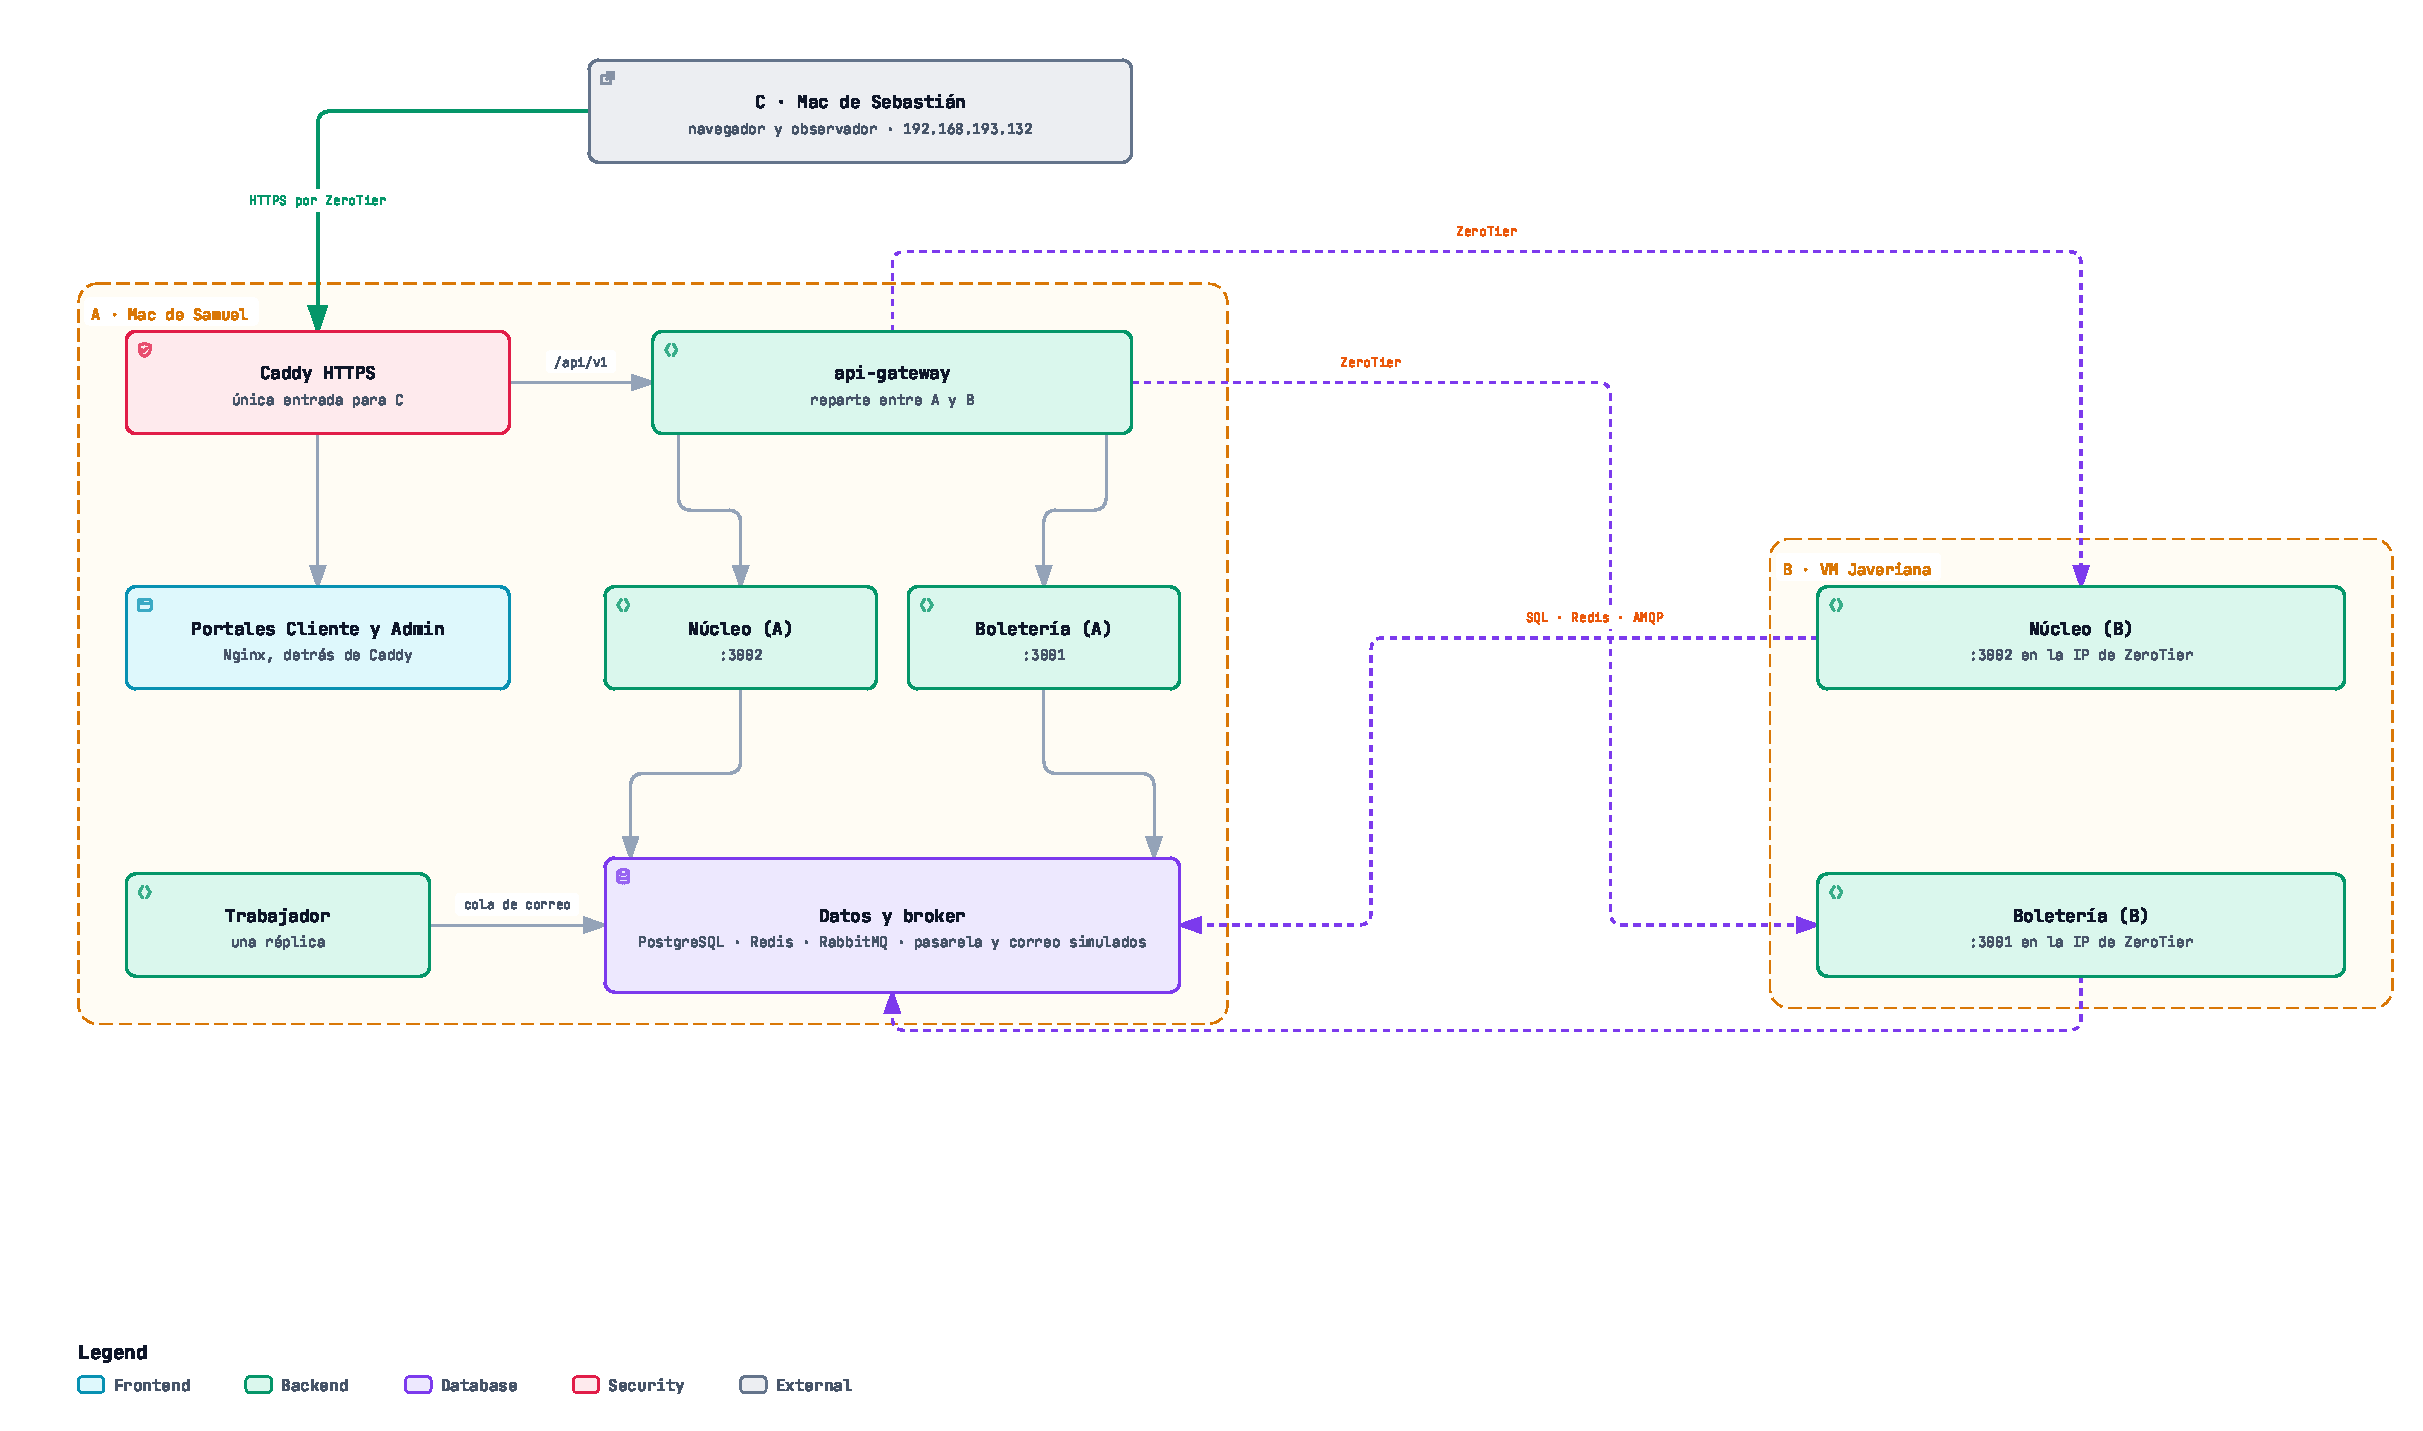
\includegraphics[width=\textwidth]{Diagrams/ArchifyPDF/09-despliegue-zerotier.pdf}
\caption{Despliegue de la demostración de disponibilidad en tres computadores.}
\label{fig:despliegue-zerotier}
\end{figure}

% ------------------------------------------------------------------
\subsection{Tiempo real y aviso de evacuación}
\label{sec:tiempo-real-vigente}

Son dos requisitos de disponibilidad en sentido amplio: que la información llegue a tiempo a quien
la necesita. RNF-09 (CU-019, CU-025) pide que un ingreso o salida se vea en el tablero en
$\leq$ 2 s. RNF-17 (CU-010) pide que una evacuación llegue a $\geq$ 99\% de los dispositivos del
personal en $\leq$ 10 s.

\begin{center}
\begin{longtable}{|>{\raggedright\arraybackslash}p{2.8cm}|>{\raggedright\arraybackslash}p{6.7cm}|>{\raggedright\arraybackslash}p{3.8cm}|}
\caption{Tácticas de tiempo real y de aviso.}\label{tab:tiempo-real-vigente}\\
\hline
\textbf{Táctica} & \textbf{Mecanismo} & \textbf{Dónde}\\
\hline
\endfirsthead
\hline
\textbf{Táctica} & \textbf{Mecanismo} & \textbf{Dónde}\\
\hline
\endhead
Empujar el estado (SSE) &
Los paneles reciben el estado por Server-Sent Events cada 1 s (antes cada 3 s, que no permitía
cumplir 2 s). Cada ciclo revalida la sesión y el permiso. &
\texttt{flujo-ocupacion.\allowbreak service.ts}, \texttt{monitoreo.\allowbreak controller.ts}\\
\hline
Mensajería asíncrona con bandeja de salida &
El ingreso por QR se guarda con su aviso en la misma transacción; la bandeja lo publica en
RabbitMQ cada 300 ms y Operación lo proyecta. La bandeja publica el lote completo y espera las
confirmaciones juntas: de unos 50 a unos 1\,700 avisos/s. &
\texttt{bandeja-salida.\allowbreak service.ts} (Acceso QR)\\
\hline
Tolerar datos incompletos &
Un ingreso sin punto de acceso se cuenta en «Acceso general»; antes iba a la cola de muertos y el
aforo del panel quedaba por debajo. &
\texttt{consumidor-\allowbreak ingresos.\allowbreak service.ts}\\
\hline
Sondeo acotado y cola de prioridad &
La app del personal consulta la evacuación activa cada 4 s; los avisos a altavoces, asistentes y
personal salen por una cola con prioridad y se reintentan cada 5 s. &
\texttt{notificador-\allowbreak evacuacion.\allowbreak service.ts}, app móvil\\
\hline
\end{longtable}
\end{center}

\paragraph{Cómo se prueba.} \texttt{tiempo-real.py} abre los paneles igual que el portal y
cronometra, para 20 ingresos por panel, desde que se envía el ingreso hasta que el panel lo
muestra; cada muestra arranca en una fase al azar del ciclo. Para RNF-17, 300 dispositivos
simulados consultan la evacuación activa cada 4 s, como la app, con las cuentas de Personal; el
organizador la propone y la confirma, y cada dispositivo anota cuándo la vio. Con
\texttt{-{}-caida}, en el instante de la activación se mata con \texttt{kill -9} una de dos réplicas
del Núcleo.

\begin{center}
\begin{longtable}{|>{\raggedright\arraybackslash}p{5.6cm}|>{\raggedleft\arraybackslash}p{1.6cm}|>{\raggedleft\arraybackslash}p{1.6cm}|>{\raggedright\arraybackslash}p{4.0cm}|}
\caption{Resultados del 16/11/2026 (\texttt{TIEMPO-REAL.md} y \texttt{TIEMPO-REAL-caida.md}).}
\label{tab:tiempo-real-resultados}\\
\hline
\textbf{Medición} & \textbf{p95} & \textbf{Máx.} & \textbf{Frente al umbral}\\
\hline
\endfirsthead
\hline
\textbf{Medición} & \textbf{p95} & \textbf{Máx.} & \textbf{Frente al umbral}\\
\hline
\endhead
RNF-09 · ingreso al parqueadero $\rightarrow$ panel CU-025 & 1,01 s & 1,01 s & 20/20 en $\leq$ 2 s\\
\hline
RNF-09 · QR en la puerta $\rightarrow$ panel CU-019 & 1,12 s & 1,12 s & 20/20 en $\leq$ 2 s\\
\hline
RNF-17 · evacuación a 300 dispositivos & 3,76 s & 3,99 s & 100\% en $\leq$ 10 s\\
\hline
RNF-17 · lo mismo, con una réplica del Núcleo muerta & 3,83 s & 4,07 s & 100\% en $\leq$ 10 s,
0 errores en 760 consultas\\
\hline
\end{longtable}
\end{center}

\paragraph{Interpretación.}
\begin{itemize}
\item \textbf{RNF-09 cumple, y la primera medición mostró por qué hacía falta cambiar.} Con un
ciclo de 3 s el peor caso ya pasaba de 2 s. Además, después de una prueba de carga de QR, 11 de
20 ingresos no llegaron al panel en 10 s: la bandeja de salida publicaba unos 50 avisos/s, esperando
la confirmación del broker de uno en uno, y tenía 19\,000 pendientes. Con las confirmaciones en
lote vació ese atraso en unos 10 s.
\item \textbf{RNF-17 cumple con margen.} El peor caso es un sondeo completo de la app (4 s) más una
respuesta; el umbral es 10 s. Matar una réplica del Núcleo al activar no cambió el resultado: el
gateway llevó las consultas a la otra.
\item \textbf{Lo que no cubre.} RNF-17 mide la llegada a la app abierta. Teléfonos sin señal o con la
app cerrada necesitan notificaciones push o SMS reales, que el prototipo no tiene. RNF-09 se midió
con carga normal: en un pico de más de 1\,700 ingresos/s la bandeja volvería a atrasarse.
\end{itemize}

% ------------------------------------------------------------------
\subsection{Monitoreo y logs}
\label{sec:monitoreo-vigente}

\begin{center}
\begin{tabular}{|>{\raggedright\arraybackslash}p{3.2cm}|>{\raggedright\arraybackslash}p{10.4cm}|}
\hline
\multicolumn{2}{|l|}{\textbf{Escenario de calidad · Monitoreo y logs (RNF-19)}}\\
\hline
Fuente & El equipo de operación durante un evento.\\
\hline
Estímulo & Necesita saber cuánta CPU y memoria usa cada instancia, cuántas réplicas están vivas y
qué dicen los logs, sobre todo durante una prueba de carga o la caída de una réplica.\\
\hline
Artefacto & Todos los contenedores del sistema y el API Gateway.\\
\hline
Entorno & Operación normal, carga y falla.\\
\hline
Respuesta & Un tablero muestra métricas y logs de todas las instancias, desde el mismo punto de
entrada que la API.\\
\hline
Medida & CPU y memoria por instancia, réplicas vivas y logs filtrables en un solo tablero, en
\texttt{/grafana/} del gateway. Muestras cada 2 s y refresco cada 5 s.\\
\hline
\end{tabular}
\end{center}

\paragraph{Diseño.} \texttt{docker-compose.monitoreo.yml} agrega cinco contenedores al sistema y se
sirve por el gateway que ya existía. No modifica los programas: ninguno tuvo que instrumentarse.

\begin{center}
\begin{longtable}{|>{\raggedright\arraybackslash}p{3.2cm}|>{\raggedright\arraybackslash}p{10.4cm}|}
\caption{Piezas del monitoreo.}\label{tab:monitoreo-piezas}\\
\hline
\textbf{Pieza} & \textbf{Qué hace}\\
\hline
\endfirsthead
\hline
\textbf{Pieza} & \textbf{Qué hace}\\
\hline
\endhead
Exportador de Docker & Lee CPU y memoria de cada contenedor de la API de Docker y las publica con
los nombres de métricas de cAdvisor (\texttt{container\_cpu\_usage\_seconds\_total},
\texttt{container\_memory\_working\_set\_bytes}).\\
\hline
Prometheus 2.55 & Guarda las métricas, con una muestra cada 2 s y 2 días de retención. Solo
conserva los contenedores del proyecto.\\
\hline
Promtail 3.2 $\rightarrow$ Loki 3.2 & Promtail recoge la salida de todos los contenedores, la
etiqueta por servicio y la envía a Loki, que la guarda y la deja consultable.\\
\hline
Grafana 11.3 & Tablero «HEXACORE · Instancias y logs», provisionado desde el repositorio (no se
configura a mano). Pide usuario y contraseña (\texttt{GRAFANA\_\allowbreak CONTRASENA} en el
\texttt{.env}): los logs muestran rutas, réplicas y errores, y el gateway lo publica a quien
llegue al puerto 8080.\\
\hline
API Gateway & Sirve Grafana en \texttt{/grafana/}: las métricas y los logs entran por el mismo punto
que la API. Además, su log de acceso registra qué réplica atendió (\texttt{upstream=}) y cuánto
tardó (\texttt{rt=}).\\
\hline
\end{longtable}
\end{center}

El tablero tiene siete paneles:
\begin{itemize}[nosep]
\item instancias vivas de gateway, Núcleo, Boletería y Trabajador;
\item CPU por instancia y memoria por instancia: cada réplica es una serie propia;
\item peticiones por réplica, sacadas del log del gateway;
\item respuestas por código HTTP;
\item latencia p95 del gateway;
\item logs de todos los servicios, filtrables por servicio.
\end{itemize}

\paragraph{Táctica y decisión.} Es la táctica de \textbf{monitorear} (detección de fallas y de
saturación). Las métricas de infraestructura salen de Docker y las de tráfico del log del gateway,
así que ningún módulo carga código de observabilidad. La propuesta inicial era usar cAdvisor, pero
no ve los contenedores con el almacén de imágenes de containerd de Docker Desktop: las versiones
0.49.1 y 0.52.1 fallan con «failed to identify the read-write layer ID» y solo informan del total
de la máquina. Por eso se escribió un exportador pequeño que lee lo mismo de la API
de Docker y publica las mismas métricas. En un Linux se puede volver a cAdvisor sin cambiar el
tablero.

\paragraph{Cómo se usa en la demostración.} El monitoreo es la evidencia visual de los otros dos
atributos:
\begin{itemize}[nosep]
\item durante la prueba de carga se ve cómo la CPU de la réplica sube hasta un núcleo y se queda
ahí;
\item al tumbar una réplica, «instancias vivas» baja, «peticiones por réplica» pasa a las réplicas
restantes, y las dos se recuperan cuando Docker la reinicia;
\item el panel de logs muestra, en el mismo lugar, el arranque de la réplica nueva.
\end{itemize}
La propia prueba de carga lee la CPU de Prometheus para su interpretación.

\paragraph{Límites conocidos.} No hay alertas automáticas: alguien tiene que mirar el tablero. La
retención es de 2 días y todo corre en un nodo, así que si la máquina cae, el monitoreo cae con
ella. Las métricas de tráfico salen del log del gateway y no de cada programa: no distinguen qué
caso de uso dentro del Núcleo consume la CPU.

% ------------------------------------------------------------------
\subsection{Trazabilidad}

\begin{center}
\begin{longtable}{|>{\raggedright\arraybackslash}p{2.6cm}|>{\raggedright\arraybackslash}p{2.2cm}|>{\raggedright\arraybackslash}p{4.4cm}|>{\raggedright\arraybackslash}p{4.4cm}|}
\caption{Del atributo a su evidencia.}\label{tab:atributos-trazabilidad}\\
\hline
\textbf{Atributo} & \textbf{RNF} & \textbf{Implementación} & \textbf{Evidencia}\\
\hline
\endfirsthead
\hline
\textbf{Atributo} & \textbf{RNF} & \textbf{Implementación} & \textbf{Evidencia}\\
\hline
\endhead
Desempeño & RNF-07, RNF-08, RNF-10 & Réplicas, balanceo con descubrimiento por DNS, pools acotados &
\texttt{prueba-carga.py}, \texttt{informe-atributos/\allowbreak CARGA-*.md}\\
\hline
Tiempo real y aviso & RNF-09, RNF-17 & SSE cada 1 s, bandeja de salida con confirmaciones en
lote, sondeo de la app y cola de prioridad & \texttt{tiempo-real.py},
\texttt{informe-atributos/\allowbreak TIEMPO-REAL*.md}\\
\hline
Disponibilidad & RNF-03, RNF-04 & Redundancia activa, reintento en el gateway, sondas de salud,
reinicio automático & \texttt{demo-\allowbreak disponibilidad.sh}, guion en
\texttt{DEMOSTRACION-\allowbreak ATRIBUTOS.md}\\
\hline
Monitoreo y logs & RNF-19 & Exportador, Prometheus, Promtail, Loki y Grafana tras el gateway &
\texttt{docker-compose.\allowbreak monitoreo.yml}, tablero \texttt{monitoreo/\allowbreak grafana/\allowbreak tableros/\allowbreak hexacore.json}\\
\hline
\end{longtable}
\end{center}
